\chapter{Introduction} 

%\subsection{\textit{Background}}
Homelessness research has undergone a significant transformation in recent years. Historically, the focus was on categorizing and describing different segments of the homeless population \citep{lee_homelessness_2021}. Much of this research has focused on individuals rather than communities. A contemporary approach views homelessness as a spectrum rather than a binary condition (e.g., Desmond et al., 2015; Swope and Hernandez, 2019; Cox et al., 2019). This paradigm shift creates opportunities to address homelessness and housing insecurity more equitably. Four critical areas remain unaddressed in the literature that limit our understanding of housing insecurity. First, housing research has concentrated on urban settings resulting in an urban-centric view of social issues like poverty and homelessness. Second, measuring housing insecurity is challenging because of its dependence on circumstances and obstacles for both individuals and communities \citep{leifheit_building_2022}. Third, housing and homelessness in urban and rural areas necessitate a multi-disciplinary approach to properly capture the aspects that contribute to them, an approach rarely used in the extant literature.  Finally, the scarcity of identified community-level risk factors in rural areas coupled with a dearth of rural-specific data and research, limits our understanding of housing insecurity and rural homelessness \citep{gleason_using_2021}. Studies on homelessness often focus on descriptive surveys of those accessing public services and providers of public services \citep{robertson_rural_2007}. Addressing these gaps by integrating rural areas into the discourse on homelessness and housing insecurity is essential for creating a just and equitable society with effective policies for preventing and addressing homelessness\citep{oregan_how_2021}.

\section{\textit{Rural Areas}}

 Rural areas encompass a broad spectrum of places, including farms, ranches, villages, forested areas, small towns, and many other qualities \citep{cromartie_defining_2008}. \citet{castle_conceptual_1998} identified a sparse population, interdependence with urban and global systems, and enormous diversity as three general characteristics of rural places.  At their core, rural areas are a function of "space, distance, and relative population density" \citep[?]{castle_place_2011}. \citet{shoup_principles_2010} group urban areas into three categories: rural areas dependent on nearby urban centers, "destination counties" with natural or artificial amenities that attract temporary residents, and production communities that revolve primarily around a single industry. This variation makes defining and understanding rurality a difficult challenge. Rural areas dominate the land mass of the United States, but with 85 percent of the population living in urban areas, they are often overlooked in the public discussion \citep{pendall_future_2016}. Despite this variation in rural areas,  "rural" is often defined as "not urban" \citep{noauthor_rural_2009}. In the study of housing, rural areas are often excluded from the conversation \citep{gkartzios_housing_2017}. Contributing to this problem is a wide variety of definitions used by governmental organizations, policymakers, and scholars (\citealp{yousey_defining_2018}; \citealp{cromartie_defining_2008}). Recently, The main policy objective for rural communities has been the promotion of economic development and preservation of the characteristics ascribed to rural areas \citep{lichter_changing_2007}. 

%While rural places take up a majority of land, 
Rural people are distributed over a blend of the rural-urban continuum. They make up about 20 percent of the nation's population, 13 percent of the metropolitan population, 48 percent of the micropolitan population, and 75 percent of the noncore-base area population \citep{isserman_national_2005}. As Figure~\ref{fig:pop_map} demonstrates, rural areas encompass a large mass of land with relatively few people compared to urban areas. Deconstructing the urban-centric lens of housing research necessitates a novel approach that can accommodate the differences in rural areas. The size and variation of rural areas necessitate addressing rural issues differently because there can be no one-size-fits-all policy approach to improving conditions for rural people. 

\begin{figure}[htbp]
    \centering
     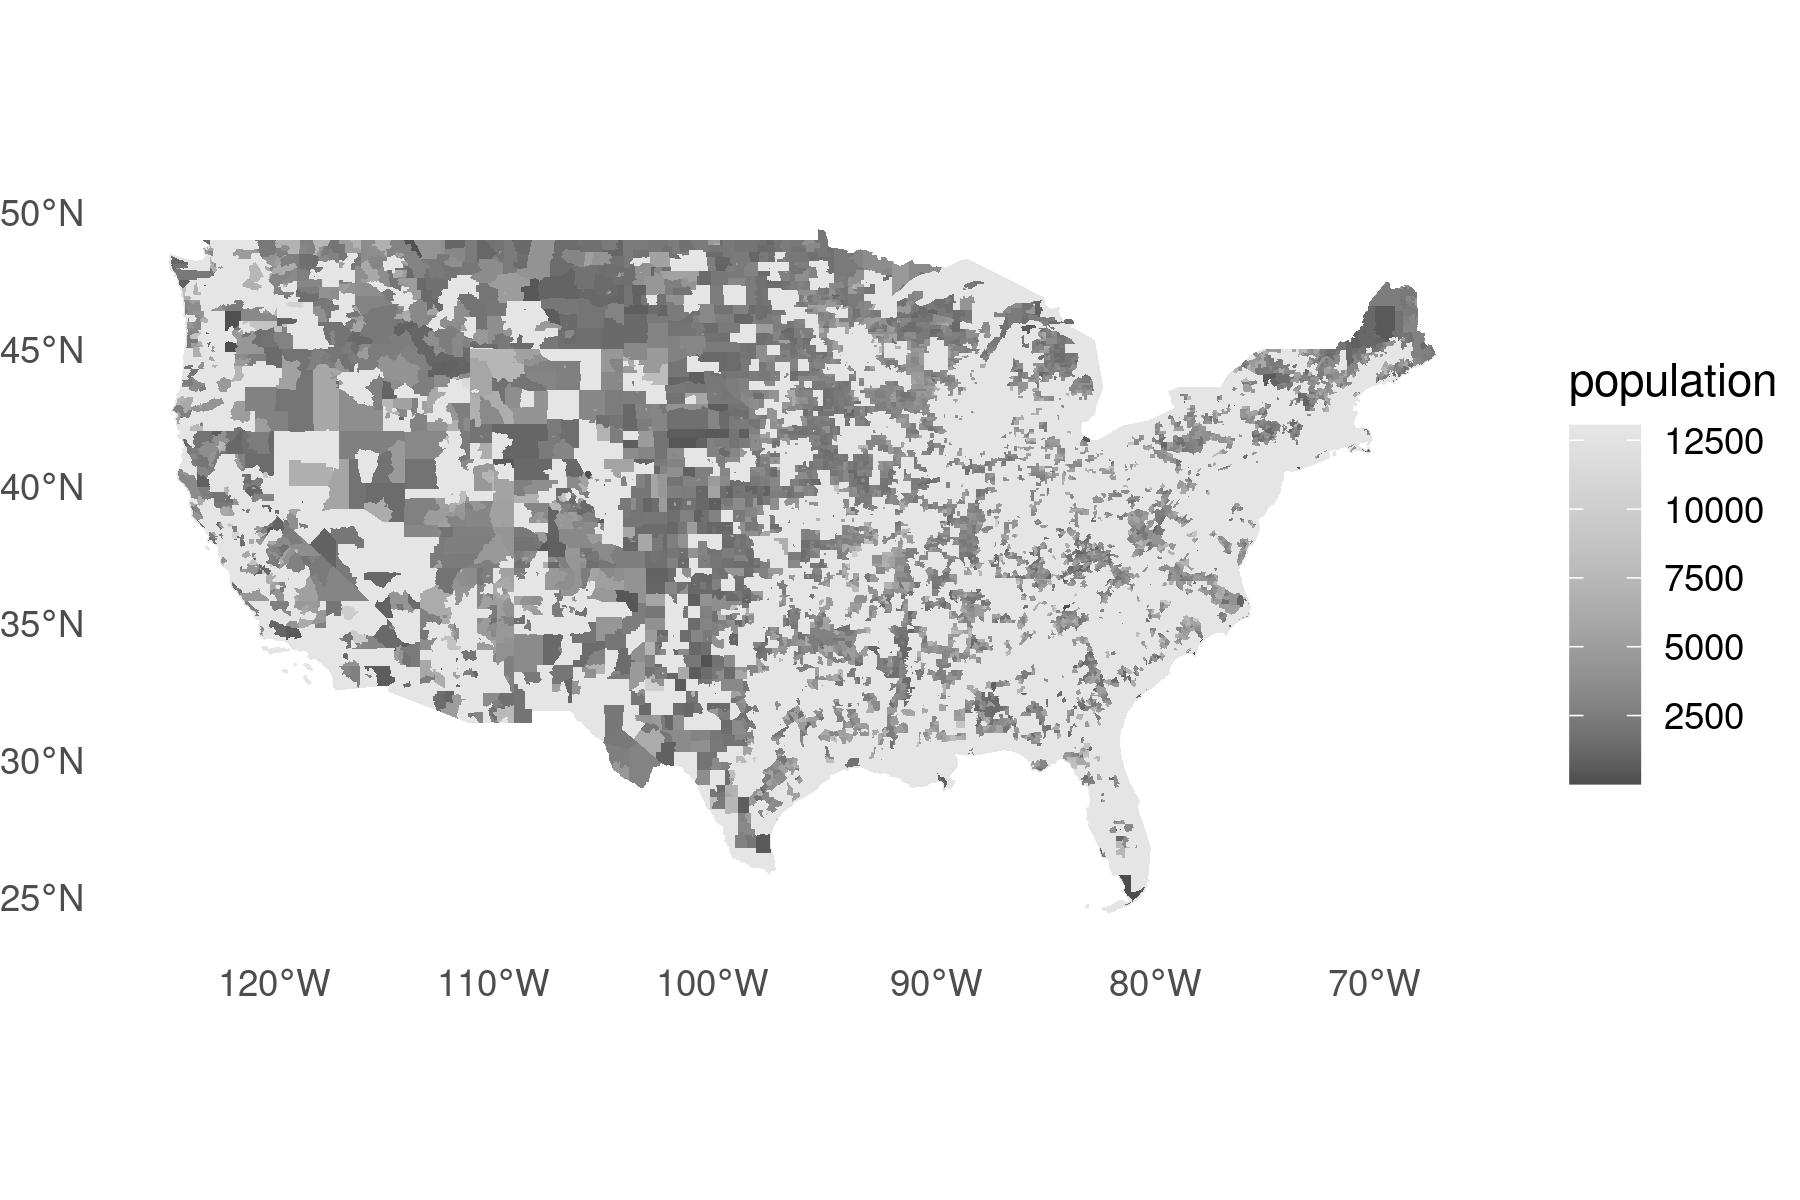
\includegraphics[width=1\textwidth, height=10cm]{plots/pop_map.png}
     \caption{Rural Population Density}
     \label{fig:pop_map}
 \end{figure}


\section{\textit{Literal Homelessness}}

For decades, scholars have debated if research should focus on the reasons why people become homeless or on the structural forces that create homelessness \citep{shlay_social_2003}. A lot of research on homelessness focused on identifying and describing categories of homeless people \citep{lee_homelessness_2021}. Researchers have also given significant attention to the binary of individuals and families being housed or unhoused and trying to assign them into umbrella categories. This neglects the wide range of individual and societal factors that occur in the phases between when a household is housed and becomes unhoused. For measuring homelessness, the most popular mechanism in the United States is the Department of Housing and Urban Development (HUD) point-in-time (PIT) count and housing inventory count. These counts are used for the distribution of federal funds for combating homelessness. As \citet{agans_enumerating_2014}  note, the unhoused frequently relocate and the housed may quickly become unhoused, making it difficult to accurately estimate the number of unhoused people at any given time. When it comes to addressing literal homelessness, public health experts differentiate between preventative services and reactive or emergency services \citep{oregan_how_2021}. Preventive services prevent households from becoming homeless, while reactive or emergency services step in after a household becomes homeless. A common reactive program is a treatment program where an unhoused person is required to participate in short-term residential programs before being placed in more permanent housing \citep{evans_reducing_2019}. As homelessness is often seen as an urban problem, most intervention occurs in urban areas \citep{gleason_using_2021}. Significant federal action on homelessness began with the passage of the McKinney-Vento Homeless Assistance Act of 1987. it provided funds to support a variety of programs  \citep{evans_reducing_2019}. The HEARTH (Homeless Emergency Assistance and Rapid Transition to Housing) Act of 2009 expanded the definitions of homelessness for supported federal programs to expand those eligible beyond the literal homeless. These included those living in a place that is not meant for habitation, people who are expected to lose their residence within 14 days, families with children that are unstably housed, and people fleeing domestic violence  \citep{evans_reducing_2019}. % need to break up the use of the same source here


\section{\textit{Housing as Health}}

A house is far more than four walls, a roof, and some doors, the characteristics and location of a house have a significant impact on one’s life. In the United States, housing is often a family’s greatest expenditure, their greatest source of wealth, and a place of safety and gathering \citep{braveman_housing_2011}. The federal government has long acknowledged this through legislation like the Housing Act of 1949, and social programs and development goals developed by HUD. Housing is often seen as one of the most fundamental determinants of health and a lack of adequate housing can produce adverse health outcomes and acts as a foundation for “social, psychological, and cultural well-being” (\citealp[p.17]{dalessandro_housing_2020}; \citealp{leifheit_building_2022}).  A health disparity or health inequity is a difference in health or health outcomes as they relate to social, political, and economic factors \citep{lutfiyya_rurality_2012}. One major factor that has been linked to health disparities is income, and this relationship exists across a wide range of socioeconomic factors \citep{canto_rural_2014}.  Part of acknowledging housing as health is moving beyond the housed and unhoused binary in order to better understand and intervene in households that are at risk of becoming unhoused. This is often referred to as housing insecurity, a broader term that encompasses a continuum that affects a larger part of the population than simply housed/ unhoused \citep{deluca_housing_2022}.

\section{\textit{Theoretical Framework}}

This thesis approaches housing from a housing insecurity perspective. Housing insecurity has a variety of definitions across government organizations, but it can be characterized as housing stability, housing affordability, housing quality/ safety, and neighborhood quality/ safety \citep{cox_road_2019}. To further refine these broad characteristics, this thesis follows the 4 C's approach to housing insecurity. With little infrastructure for homelessness services in rural areas, the 4 C’s approach to housing insecurity proposed by \citet{hernandez_housing_2019} can highlight areas of critical concern for devoting resources to reactive services and identify areas where preventative services can improve or expand. The pillars of the 4 C's include conditions: the quality of housing, cost: the affordability of housing, consistency: residential stability, and context: neighborhood opportunity. The 4 C’s of housing are an interconnected web of factors that impact health and encapsulate the “unequal distribution of housing disparities along other axes of inequality, and the historical forces shaping unequal housing opportunities” \citep[1]{hernandez_housing_2019}.  Swope and Hernandez are not the only scholars to design a model encompassing these 4 factors. \citet{metzger_fair_2017} proposed a similar framework that encompasses stability, affordability, internal housing conditions, and area characteristics. That multiple scholars have conceptualized a similar approach indicates that it may appropriately encapsulate housing insecurity within the limitations of our understanding. 

\section{\textit{Motivation}}
Three primary reasons motivate this thesis:

The first motivation stems from the lack of attention scholars have paid to rural areas as it pertains to housing insecurity. While the literature on rural housing insecurity is growing, there has yet to be a holistic nationwide survey of rural housing insecurity. Rural areas deserve more attention, and this thesis hopes to serve as a starting point for future research on rural housing insecurity at all levels with the ultimate goal of breaking the urban-focused lens of housing insecurity. The second motivation is to provide an implementation of the 4 C's model of housing insecurity in the rural United States. With the urban lens to housing insecurity, an adequate theoretical model must be capable of adapting to areas often left out of the conversation. One study \citep{gleason_using_2021} has applied the 4 C's model to housing insecurity in the state of Maine. Most applications of the 4 C's have been to study the relationships between various conditions and housing insecurity, but no studies have applied it broadly to rural housing insecurity at the community level. The final motivation is to provide policy-makers and researchers with a framework to identify rural areas of housing insecurity in their constituency and create harm reduction approaches and services that can meet the unique needs of their areas. The patchwork of local, state, and federal systems that encompass the aid programs of the United States means that many people are involved in the policy-making process with no adequate mechanism for addressing housing insecurity in their constituency.

\section{\textit{Approach}}

In order to improve our understanding of rural housing insecurity, this thesis investigates the risk levels of rural census tracts in the United States under the 4 C's model of housing insecurity. Risk factors across eight different axes are used to assign risk levels to rural census tracts. Each state is clustered with census tracts from other states within a 15-mile boundary to encapsulate how communities span across state lines. The cluster medians are analyzed to understand the trends in housing insecurity factors across states and the clusters are relabeled based on risk factors identified in the literature so that each cluster falls into a low, medium, or high-risk level. These risk levels are used to highlight census tracts at a low, medium, and high risk of housing insecurity relative to other census tracts in their state. Association rules learning is used to identify common patterns between sector risk levels and identify pockets of rural census tracts that are at high risk of housing insecurity. To better understand how factors of housing insecurity relate to space, Moran's I spatial autocorrelation is used to determine how spatially clustered each housing insecurity factor is. Local Moran's I is used to determine how spatially clustered each risk level is to better understand the clustering of housing insecurity risk in rural areas. Finally, a multinomial logistic regression is used to determine how well each state's sector risk levels can be predicted, and a national model is generated for each sector's risk levels to analyze well the risk levels created by this implementation of the 4 C's model can be predicted nationally and state by state. 

Beginning to understand rural homelessness requires that several questions be answered: How can risk factors be used to identify risk levels of housing insecurity while accounting for the variation in rural areas and what do the risk levels say about rural areas? When measuring housing insecurity across different dimensions, how often do the same features arise? Are there spatial relations between the different dimensions of housing insecurity? To what extent can this model of housing insecurity be used to predict risk levels across housing insecurity factors?

\section{\textit{Major Results}}

The work presented in this thesis presents a novel application of the 4 C's of housing insecurity framework and applies it to rural areas. This framework allows for the identification of 776 rural census tracts with a high or medium risk of housing insecurity. The association rules learning results shows that there are a notable amount of unexpected relationships where a high risk in one sector is associated with a low risk in another sector and vice versa. It also presents evidence that clustering of housing insecurity factors may not be as common in rural areas as they are in urban areas. It also shows that it is difficult to predict the risk levels of census tracts with state and national models. Due to its exploratory nature, the results are primarily intended to be used as a starting point for future research into rural housing insecurity. 

\section{\textit{Intended Audience}}
This thesis is intended for an audience with a significant interest in rural housing insecurity. Such an audience can include but is not limited to policymakers, economists, political scientists, community psychologists, rural sociologists, and many others concerned with housing insecurity and rural areas. 

\section{\textit{Structure of Thesis}}
The thesis is structured into six chapters. Chapter 2 offers a comprehensive theoretical foundation, focusing on the application of the 4 C's of the housing insecurity model. This chapter reviews pertinent literature on various facets of the model. Chapter 3 explains the methodology employed for data processing. It provides an in-depth explanation of the methodology for applying the theoretical framework and its execution. Chapter 4 presents the study's findings, offering a detailed analysis of the acquired results. Chapter 5 deliberates on the results, discussing their significance and impact within the scope of the study. This chapter provides a thorough examination of the noteworthy findings. Chapter 6 serves as a synthesis, summarizing the entirety of the work and offering insightful commentary on the major findings. Additionally, it highlights potential avenues for future research and study.

\endinput